%%%%%%%%%%%%%%%%%%%%%%%%%%%%%%%%%%%%%%%%%
% University Assignment Title Page 
% LaTeX Template
% Version 1.0 (27/12/12)
%
% This template has been downloaded from:
% http://www.LaTeXTemplates.com
%
% Original author:
% WikiBooks (http://en.wikibooks.org/wiki/LaTeX/Title_Creation)
%
% License:
% CC BY-NC-SA 3.0 (http://creativecommons.org/licenses/by-nc-sa/3.0/)
%%%%%%%%%%%%%%%%%%%%%%%%%%%%%%%%%%%%%%%%%

\documentclass[12pt]{article}
\usepackage[english]{babel}
\usepackage[utf8x]{inputenc}
\usepackage{amsmath}
\usepackage{graphicx}
\usepackage[colorinlistoftodos]{todonotes}
\usepackage{float}

\begin{document}

\begin{titlepage}

\newcommand{\HRule}{\rule{\linewidth}{0.5mm}}

\center

\textsc{\LARGE Politenico di Milano}\\[1.5cm]
\textsc{\Large Dipartimento Elettronica, Informazione e Bioingegneria}\\[0.5cm]
\textsc{\large HEAPLab Project Report}\\[0.5cm] 

\HRule \\[0.4cm]
{ \huge \bfseries I2C LCD2004 display driver for Miosix OS}\\[0.4cm]
\HRule \\[1.5cm]

\begin{minipage}{0.4\textwidth}
\begin{flushleft} \large
\emph{Author:}\\
Emanuele \textsc{Pisano}
\end{flushleft}
\end{minipage}
~
\begin{minipage}{0.4\textwidth}
\begin{flushright} \large
\emph{Supervisor:} \\
Dr. Federico \textsc{Terraneo}
\end{flushright}
\end{minipage}\\[2cm]

{\large \today}\\[2cm]


\includegraphics[width=100pt]{heaplogo.pdf}\\[1cm]
 
\vfill

\end{titlepage}




\begin{abstract}
Development and implementation of a driver for the I2C LCD2004 display to be installed on MiosixOS
\end{abstract}

\section{Introduction}

The I2C LCD2004 is a liquid crystal display that, thanks to the integration with a PCF8574T remote 8-bit I/O expander, is capable of using I2C (Inter Integrated Circuit by Philips) to connect to a controller, greatly reducing the number of occupied board IOs but still providing good performance. Indeed, I2C requires only two bidirectional signal lines (Serial Data Line (SDA) and Serial Clock Line (SCL)), plus two more IOs for power supply. Furthermore, more than one device can be connected in series through this bus.
The aim of this project is to design and implement a Miosix OS driver for this device.


\section{Design and Implementation}

\subsection{Premise: the product and the PCF8574T remote 8-bit expander}
Good part of the effort spent in the project was required to fully understand how the device works in its completness. As already said, the device is composed by the union of 2 devices: the LCD2004 liquid crystal display and the PCF8574T remote 8-bit I/O expander. The documentation for these 2 devices as standalone is good and easily retrievable. However, when it comes to the final product there is no documentation that explains how they are connected and work together. In order to fully understand this, I often had to do some reverse-engineering.
Hereinafter, a brief explanation of the PCF8574T remote 8-bit I/O expander:
the device is what allows the LCD to receive data from the I2C bus as if they were sent over 13 parallel IOs. It receives 8 bit at time, following the I2C protocol (addressing, start/stop signaling, acknowledgements, etc...) accumulating  them in a shift register. Once collected them, it sends them in parallel to the LCD2004. One of the problems that I managed to resolve only by reverse-engineering the device was: how 13 IOs could be substituted by 8? I discovered then that the PCF8574T exploits the 4-bit mode of the LCD2004, that basically tells the display to only use 4 of the 8 data input IOs. Using only 4 bits to send data, the remaining 4 are connected to 4 command pins on the LCD2004. At the end, only 1 of the 13 IOs of the display is not connected, but this does not represent a big issue, since the majority of the display's funcions can be used without it. So, as it will be clear when reading the implementation, every byte sent to the PCF8574T is composed by 4 bits of data and 4 bits for commands, that must be set to the exact value during every trasmission (one for the backlight, one for the enable signal, and the last two to represent the message mode).

\subsection{Design}
The aim of the driver is to provide a simple interface to the user by using simple methods, in order to make transparent all the underlying details.
At the very lower level there is an instance of the singleton class "I2C1Driver" (already implemented in the Miosix kernel) responsible for all the trasmission and protocol details over the I2C bus. This is used by the method "send" to send correctly "encoded" 8 bits to the device.
At the next level, the method "send4bits" sends 4 bits of (pure) data, and beside it the method "sendEnable" sends the enable signal, required by the PCF8574T to correctly interpret the message.
Above them, the method "send8bits" sends 8 bits, being either commands or a character to write. To send command, the relative bit has to be set to 0, and this is automatically done by the method "sendCommand".
At the highest level there are all the methods provided for the user, with intuitive names so that often no explanation is required to understand what they do.
\begin{figure}
\centering
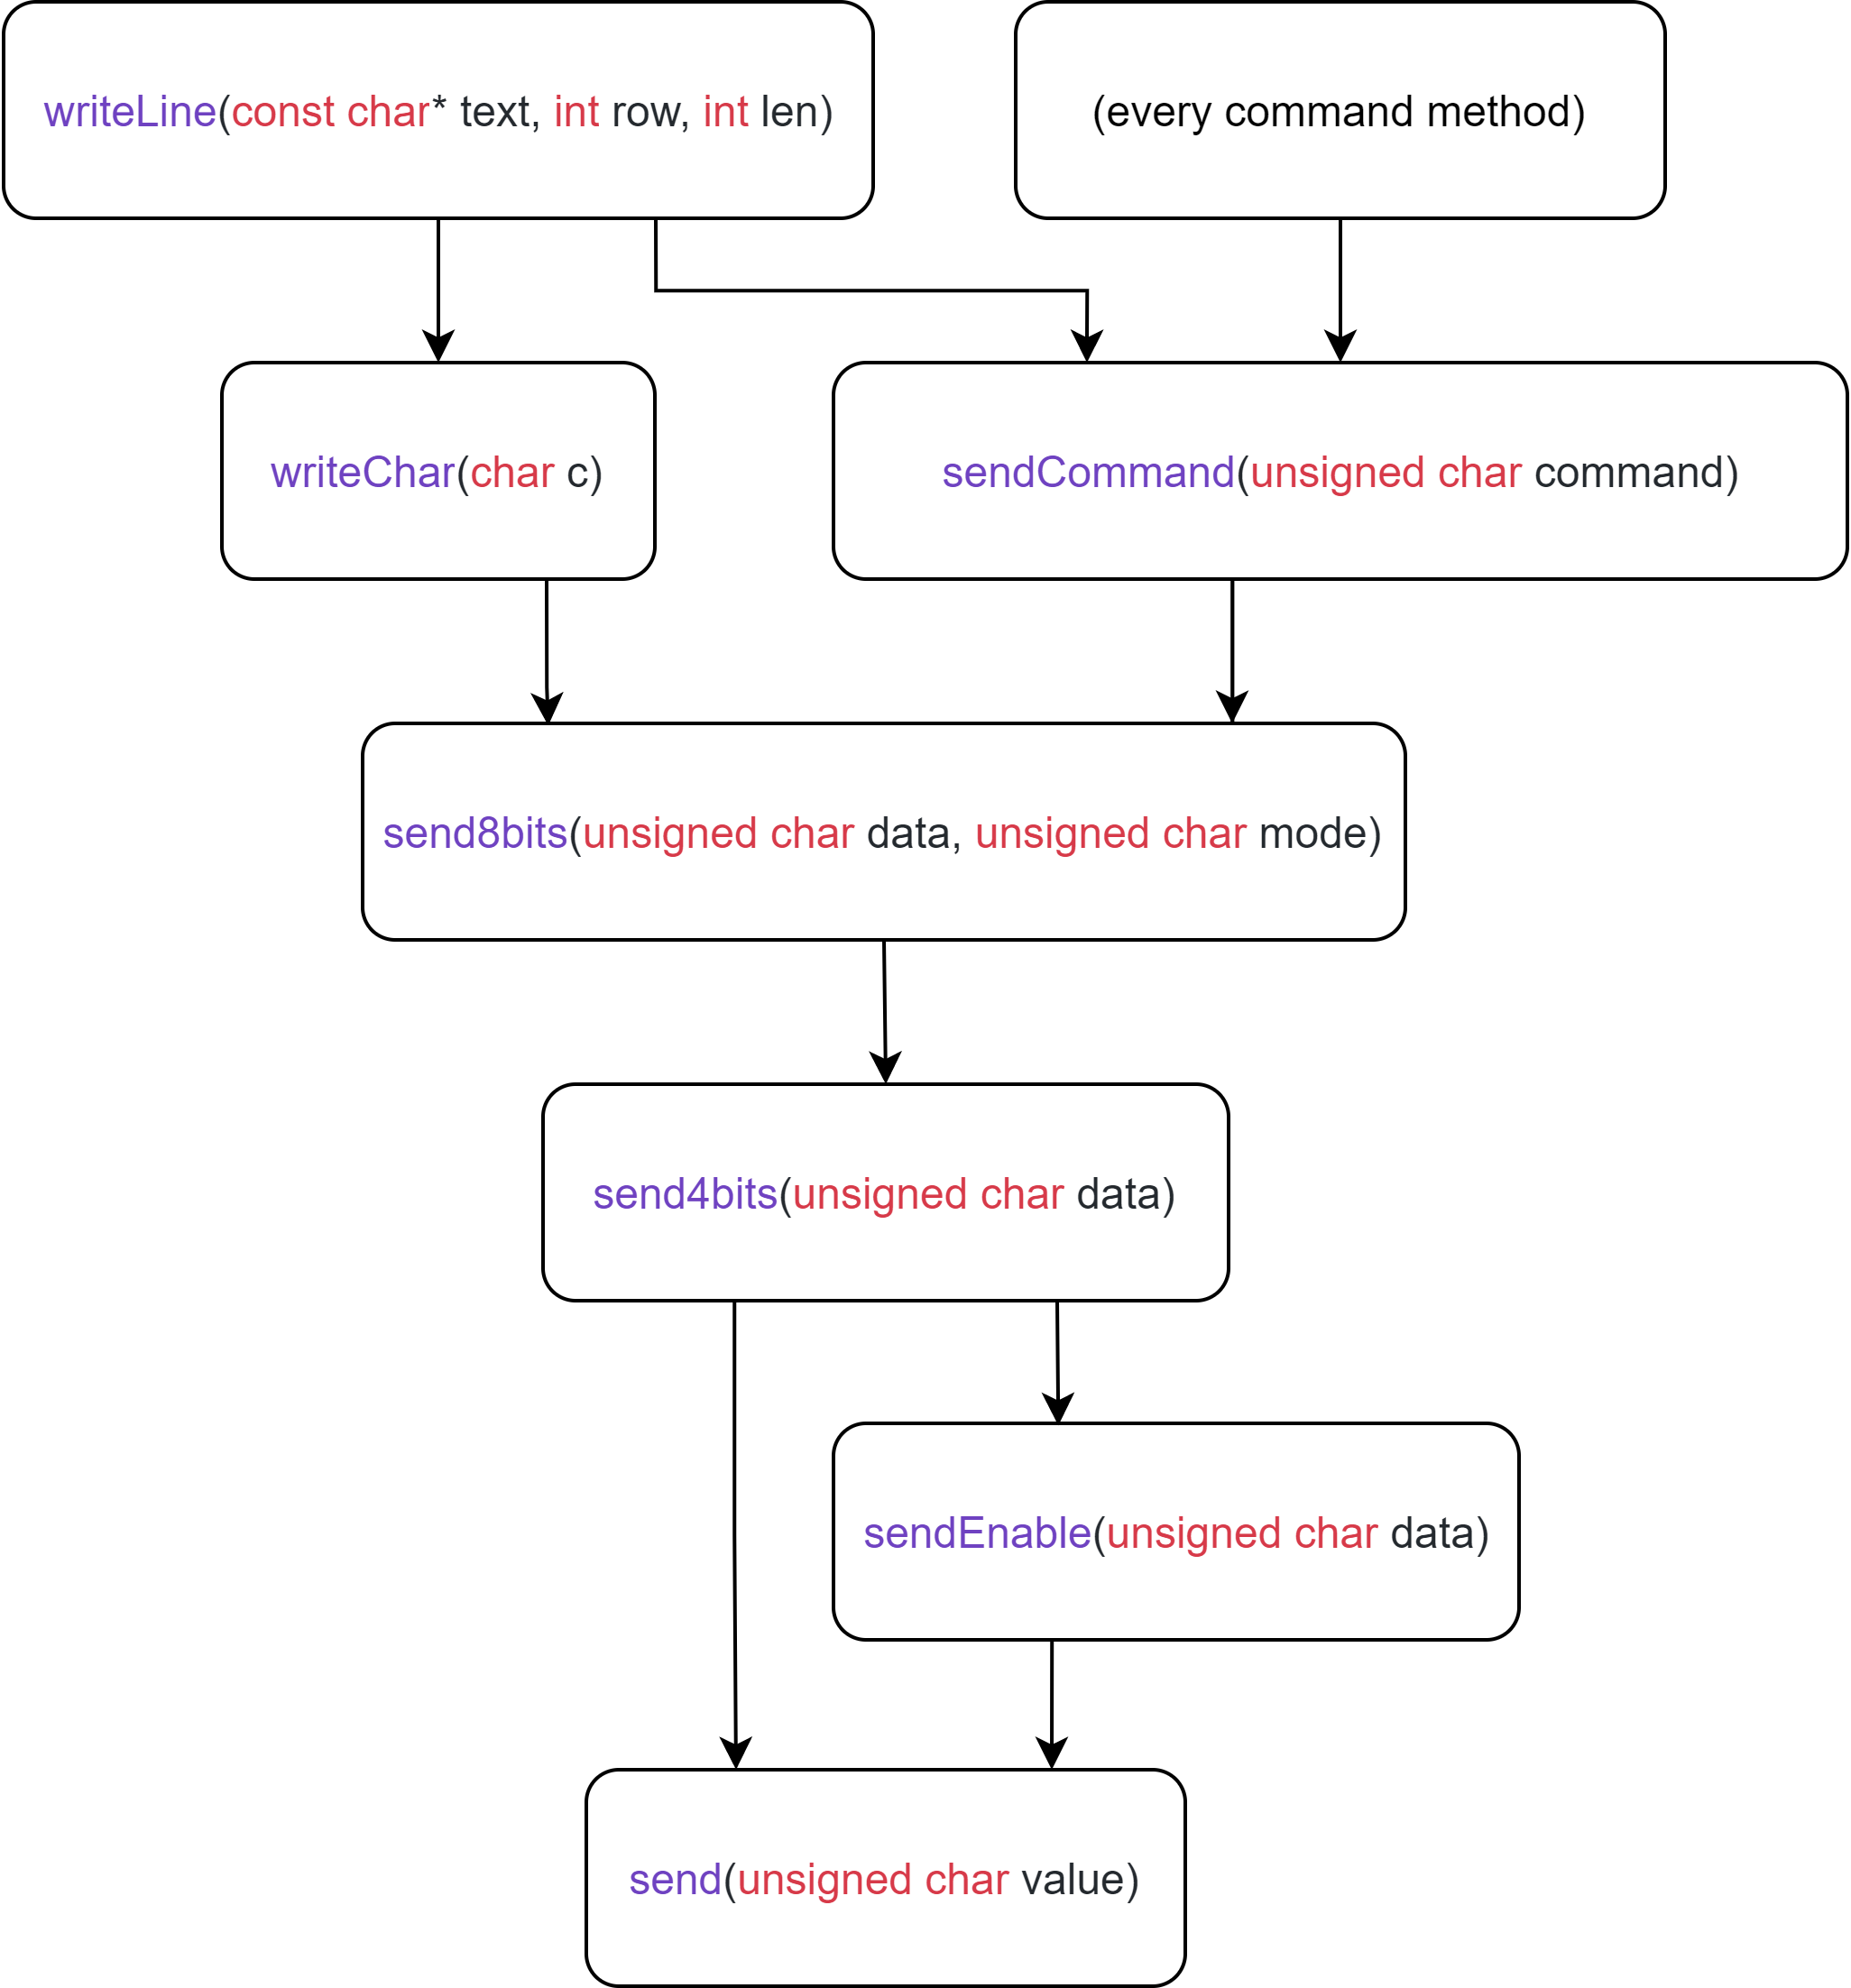
\includegraphics[width=0.55\textwidth]{diagram.png}
\caption{\label{fig:}Diagram representing functions calls.}
\end{figure}

\vfill

\subsection{Implementation}
All the methods except the constructor and init() return a boolean value expressing the result of the operation (true on success, false on failure).
Follow a list of all the methods, plus a brief explanation for the ones not very trivial:

\begin{itemize}

\item Lcd2004(GpioPin scl, GpioPin sda, unsigned char address, int columns, int rows): constructor of the class, requires the 2 pins to be used as Serial Clock and Serial Data, the address of the device and number of rows and columns it provides.
It sets all the class fields, configures the Gpios and initializes the device calling init()

\item init(): correctly initializes the device by sending a specific series of bits that basically tells it to use the 4-bit interface mode to communicate from that point onwards. Plus, the device configuration is set to the basic configuration, that can be modified later.

\item clear(): clears completely the screen

\item home(): sets the cursor to the home position (0,0)

\item setPosition(int column, int row): sets the cursor to the specified position

\item writeChar(char c): writes a char in the actual cursor position (then the cursor position is automatically increased by one by the device itself)

\item writeLine(const char* text, int row, int len): writes the first "len" character from the given "text" in the given "row". This method should simplify writing more than 1 character at a time. If no len is specified, the full text will be written.

\item displayOn() and displayOff(): turns on/off the display

\item backlightOn() and backlightOff(): turns on/off the backlight

\item cursorOn() and cursorOff(): turns on/off the cursor

\item blinkOn() and blinkOff(): turns on/off the blinking cursor

\item scrollRight() and scrollLeft(): scrolls display right/left

\item entryRight() and entryLeft(): sets entry mode to right/left

\item alignRight() and alignLeft(): aligns text right/left

\item sendCommand(unsigned char command): sends 8 bits setting correctly the command bit

\item send8bits(unsigned char data, unsigned char mode): sends 8 bits in the specified mode (command or write) breaking them in 2 chunks of 4 bits.

\item send4bits(unsigned char data): sends 4 bits of data followed by an enable signal to validate them

\item sendEnable(unsigned char data): sends an enable signal to validate data just sent

\item send(unsigned char value): sends 8 bits through the I2C bus using I2C1Driver class

\end{itemize}



\section{Experimental Results}
In its final implementation the driver with all its methods is correctly working. Here some images with the aim of showing some of its functions:

\begin{figure}[H]
\centering
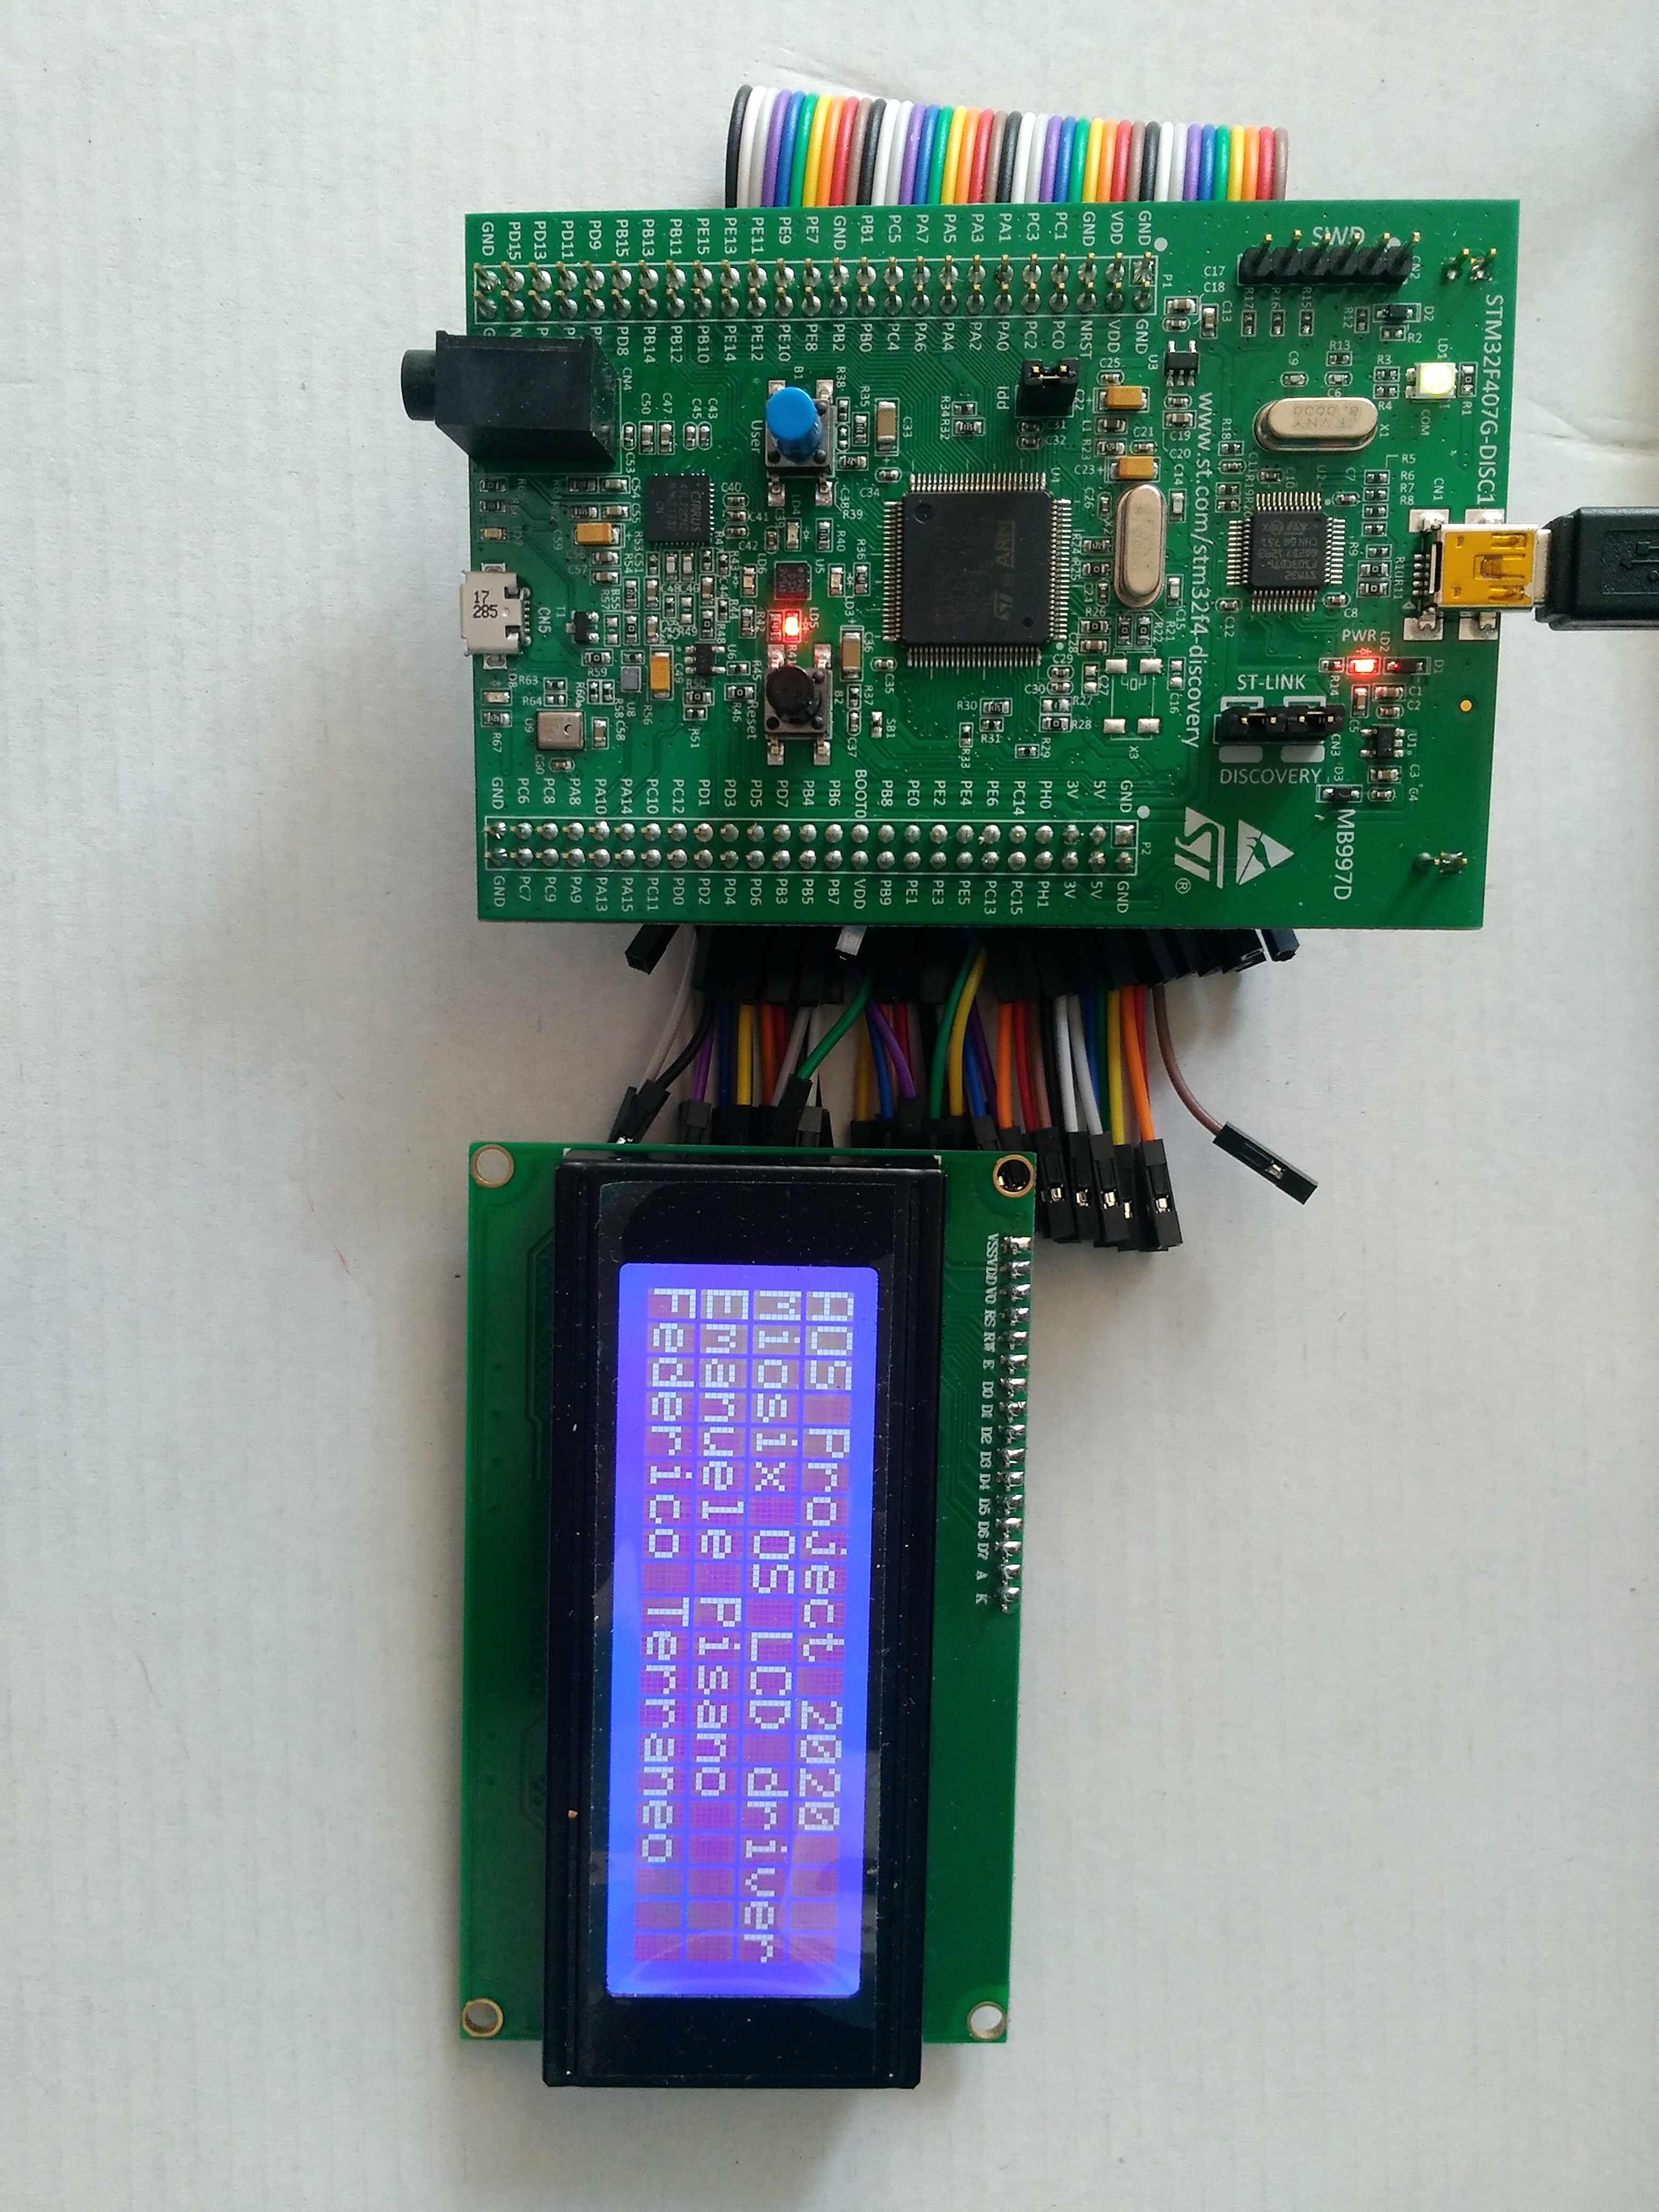
\includegraphics[width=0.5\textwidth, angle=90]{foto_normale.jpg}
\caption{\label{fig:}Multiple lines written with writeLine method.}
\end{figure}

\begin{figure}[H]
\centering
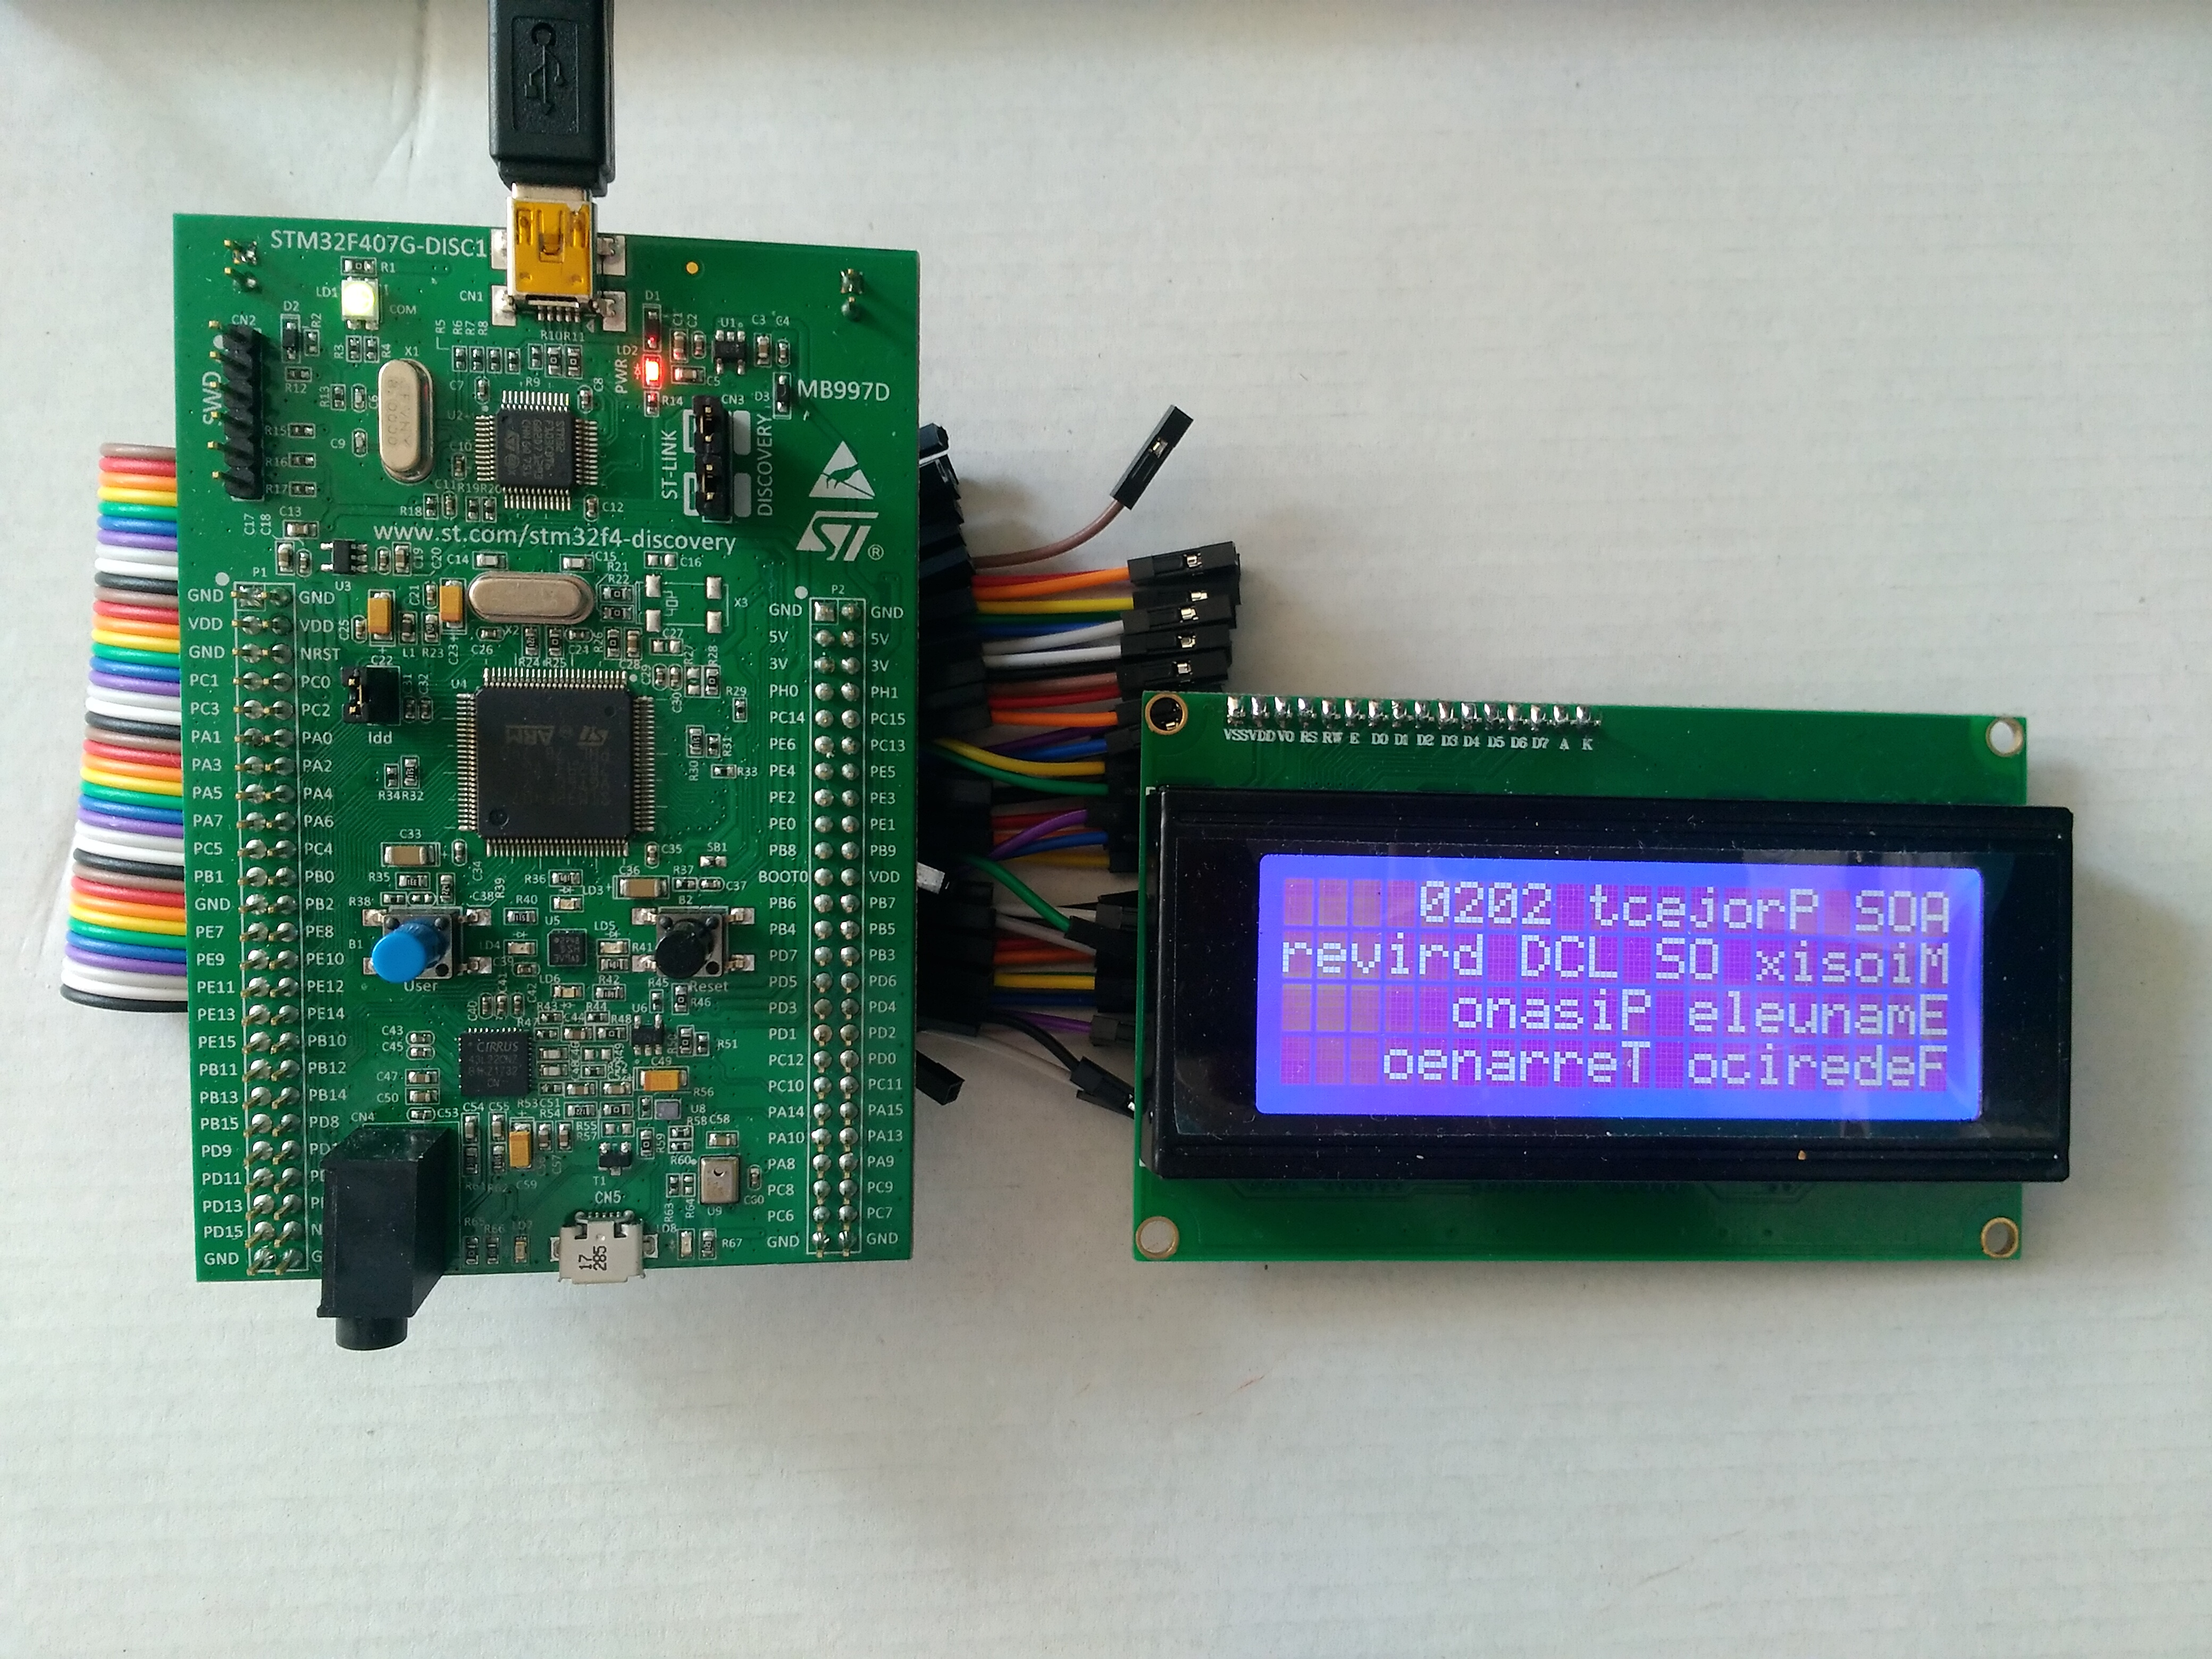
\includegraphics[width=0.68\textwidth]{foto_entry_right.jpg}
\caption{\label{fig:}Multiple lines written in right-entry mode.}
\end{figure}

\begin{figure}[H]
\centering
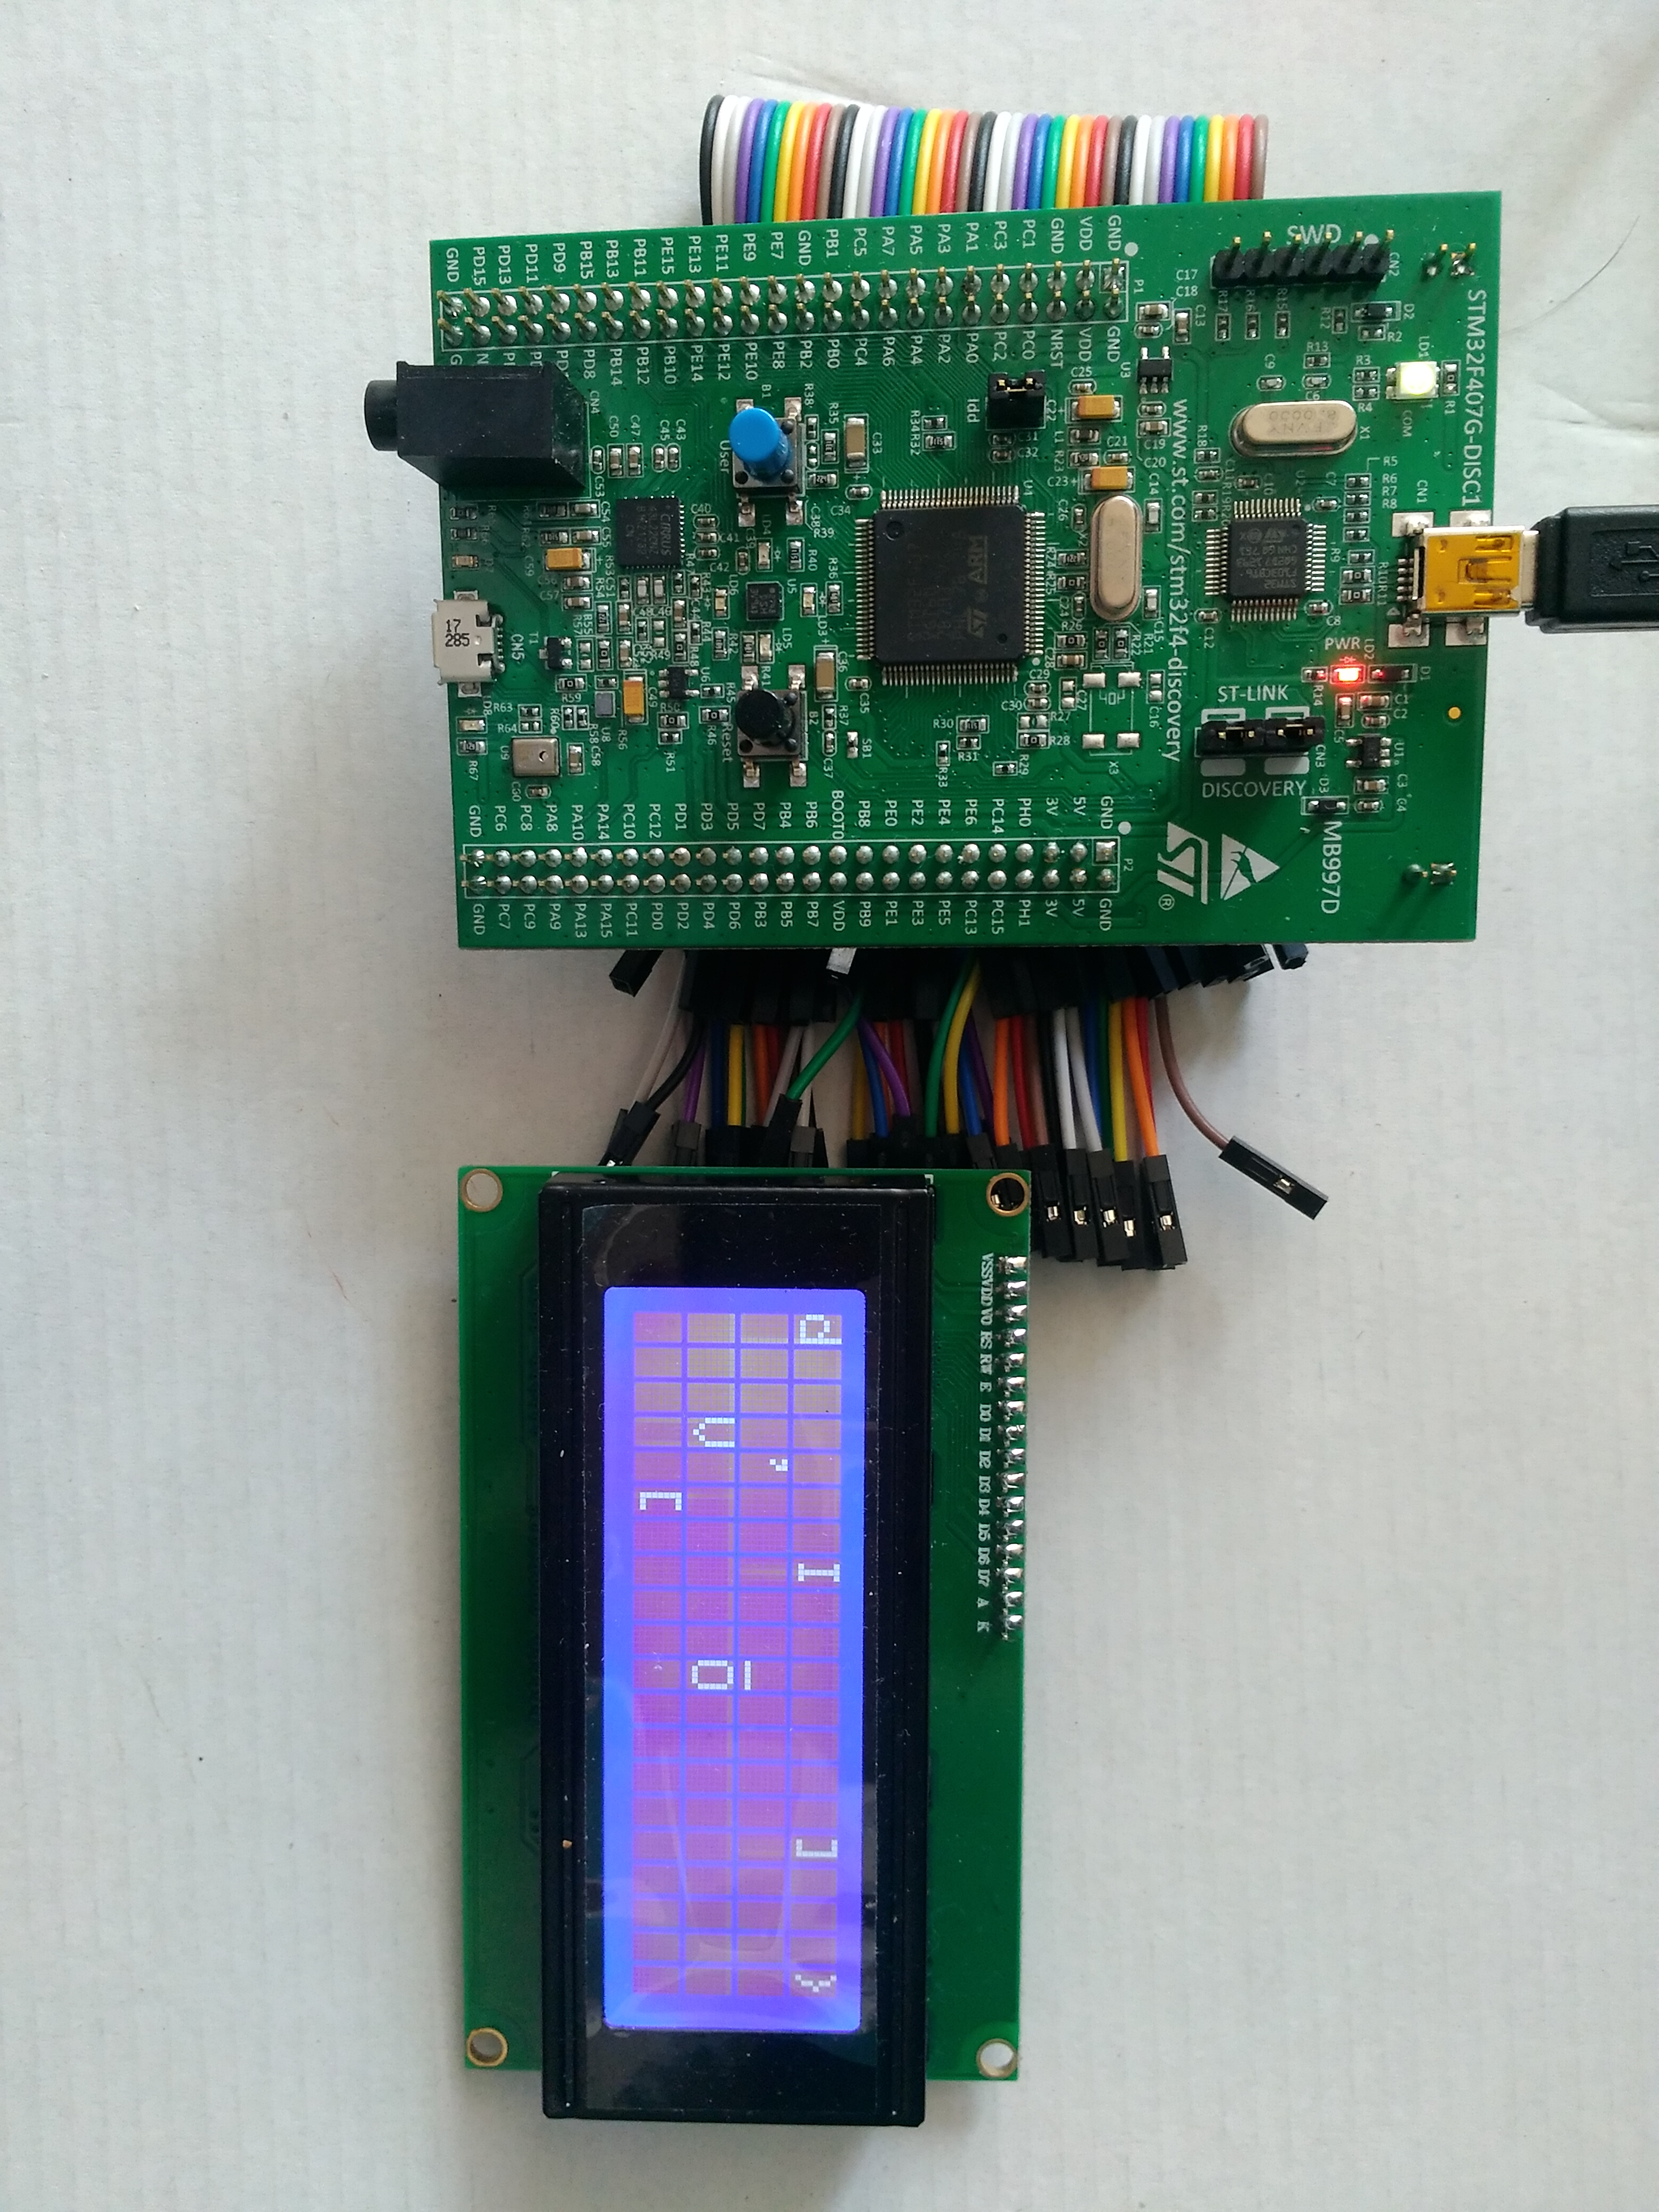
\includegraphics[width=0.5\textwidth, angle=90]{foto_random_char.jpg}
\caption{\label{fig:}Random characters written in random positions using writeChar and setPosition methods.}
\end{figure}

\begin{figure}[H]
\centering
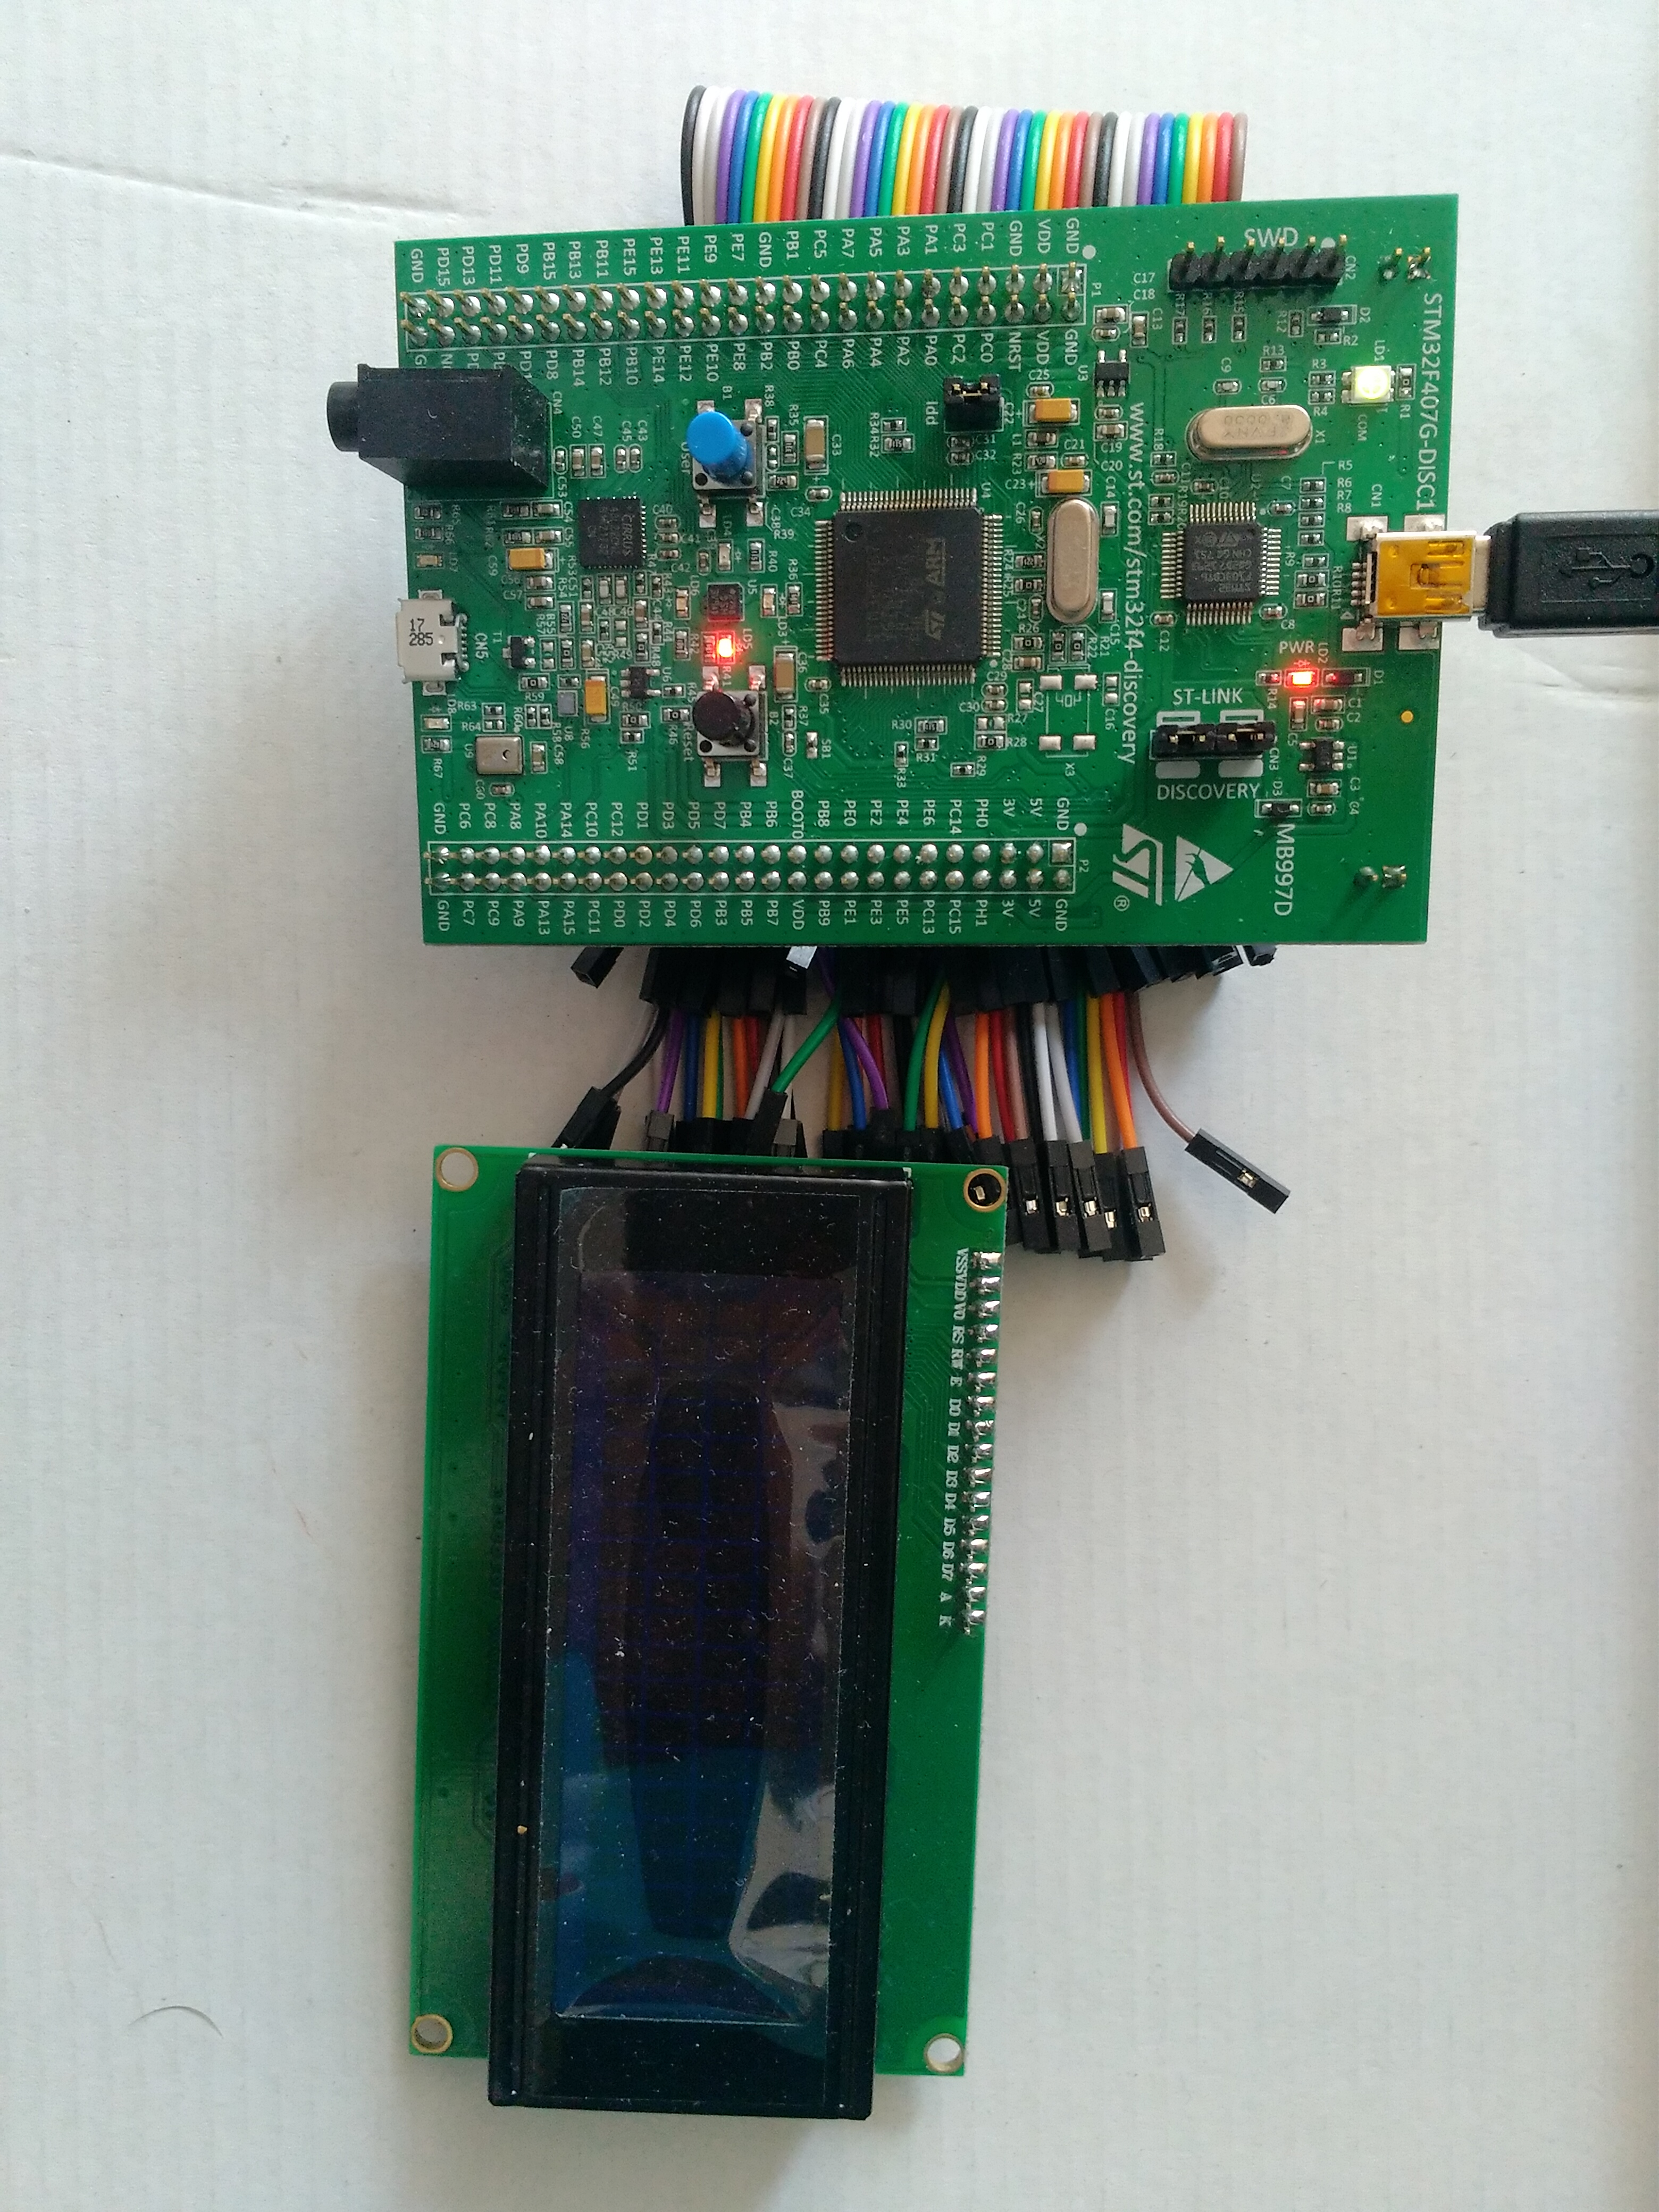
\includegraphics[width=0.5\textwidth, angle=90]{foto_off.jpg}
\caption{\label{fig:}displayOff method works :-)}
\end{figure}

\vfill

\section{Conclusions}
The driver implemented is working and could be added to the standard Miosix common drivers, hopefully simplifying the usage of the device for various purposes.

\end{document}
